\documentclass[11pt]{beamer}
\usetheme{Copenhagen}
\usepackage[utf8]{inputenc}
\usepackage[english]{babel}
\usepackage{amsmath}
\usepackage{amsfonts}
\usepackage{amssymb}
\usepackage{graphicx}
\usepackage{caption}
\usepackage{subcaption}
\DeclareMathOperator{\argmin}{\mathrm{arg\, min}}
\author{Onofre Martorell, Lidia Talavera}
\title{Image inpainting}
%\setbeamercovered{transparent} 
%\setbeamertemplate{navigation symbols}{} 
%\logo{} 
%\institute{} 
%\date{} 
%\subject{} 
\begin{document}

\begin{frame}
\titlepage
\end{frame}

%\begin{frame}
%\tableofcontents
%\end{frame}

\begin{frame}{From functional to Laplace equation}
We have the functional
$$
\displaystyle\argmin\limits_{u\in W^{1,2}(\Omega)}\int _D |\nabla u(x)|^2dx
$$
According to the Necessary condition for the extremum\footnote{We saw this result at the first class of the module}, the minimum of the functional is the solution of
$$-\sum_{i=1}^2 \frac{\partial}{\partial x_i}\frac{\partial\mathcal{F}}{\partial p_i} + \frac{\partial\mathcal{F}}{\partial u} = 0$$

where $\nabla u(u) = (p_1, p_2)$ and $\mathcal{F}$ is the function inside the functional.
\end{frame}

\begin{frame}{From functional to Laplace equation}
Replacing the given functional, we get
$$ 0 = - \frac{\partial}{\partial x}\frac{\partial(u_x^2 + u_y^2)}{\partial u_x} - \frac{\partial}{\partial y}\frac{\partial(u_x^2 + u_y^2)}{\partial u_y} + \frac{\partial(u_x^2 + u_y^2)}{\partial u} = $$
$$ = - \frac{\partial}{\partial x}(2u_x) - \frac{\partial}{\partial y}(2u_y) + 0 = 2u_{xx} + 2u_{yy}$$
In conclusion,
$$2(u_{xx} + u_{yy})=0\Longrightarrow \Delta u = 0$$
\end{frame}

\begin{frame}{The problem of inpainting}
The problem of inpainting can be modelled as
$$
\begin{cases}
\displaystyle\argmin\limits_{u\in W^{1,2}(\Omega)}\int _D |\nabla u(x)|^2dx,\\
u|_{\partial D} = f
\end{cases}
$$
where $f$ is the image to inpaint.


With the result obtained, this problem is equivalent to find the solution of
$$\left\lbrace
\begin{array}{l l}

\Delta u = 0& \text{in }D \\
u = f & \text{in }\partial D

\end{array}\right.
$$
The equation is completed with homogeneous Neumann boundary
conditions at the boundary of the image.

\end{frame}

\begin{frame}{Discretization of the laplacian}
The laplacian can be computed as
$$\Delta u = div(\nabla u).$$

\begin{block}{Discretization of the gradient}
Using forward differences, we obtain
$$\nabla u_{ij} = \bigg(\frac{u_{i+1,j} - u_{i,j}}{h_i}, \frac{u_{i,j+1} - u_{i,j}}{h_j}\bigg)$$
\end{block}
\begin{block}{Discretization of the divergence}
Taking $v = (v_1, v_2)$ and using backward differences, we obtain
$$div(v)_{i,j} = \frac{v_{1_{i,j}} - v_{1_{i-1,j}}}{h_i} + \frac{v_{2_{i,j}} - v_{2_{i,j-1}}}{h_j}$$
\end{block}
\end{frame}

\begin{frame}{Discretization of the laplacian}
Joining the previous discretizations and doing some calculus we obtain the following equation for each pixel in $D$
$$\frac{1}{h_j^2}u_{i,j-1} + \frac{1}{h_i^2}u_{i-1, j} - \bigg(\frac{2}{h_i^2}+\frac{2}{h_j^2}\bigg)u_{i,j} + \frac{1}{h_i^2}u_{i+1,j} + \frac{1}{h_j^2}u_{i, j+1} = 0$$


\end{frame}

\begin{frame}{Boundary conditions}
For the boundary of the image we have added one row or column to each side of the image and we have computed the Neumann boundary conditions. For example, at the east side, we get
$$\frac{u_{i, 1} - u_{i, 2}}{h_j} = 0\Longrightarrow u_{i,1} = u_{i, 2}$$

\end{frame}

\begin{frame}{System of equations}
To sum up, we have an equation for each type of pixel in the image
\begin{itemize}
\item Pixels belonging to $D$:
$$\frac{1}{h_j^2}u_{i,j-1} + \frac{1}{h_i^2}u_{i-1, j} - \bigg(\frac{2}{h_i^2}+\frac{2}{h_j^2}\bigg)u_{i,j} + \frac{1}{h_i^2}u_{i+1,j} + \frac{1}{h_j^2}u_{i, j+1} = 0$$
\item Pixels not belonging to $D$:
$$u_{i, j} = f_{i, j}$$
\item Pixels on the boundary:
$$u_{i,1} = u_{i, 2},\ u_{i,n_j} = u_{i, n_j-1},\ u_{1,j} = u_{2, j}\ \text{or } u_{n_i,j} = u_{n_i-1, j},$$
depending if the pixel belongs to east, west, north or south boundary.
\end{itemize}
\end{frame}

\begin{frame}{System of equations}
Ordering the pixels of the image as
$$x = (u_{1,1}, u_{2,1}, \cdots, u_{i, j}, u_{i+1, j}, \cdots ,u_{n_i + 2,n_j + 2})^T$$
the previous equations can be written as a linear system of equations 
$$Ax = b,$$
which can be solved using Matlab.
\end{frame}

\begin{frame}{Results}

\begin{figure}
    \centering
    \begin{subfigure}[b]{0.5\textwidth}
        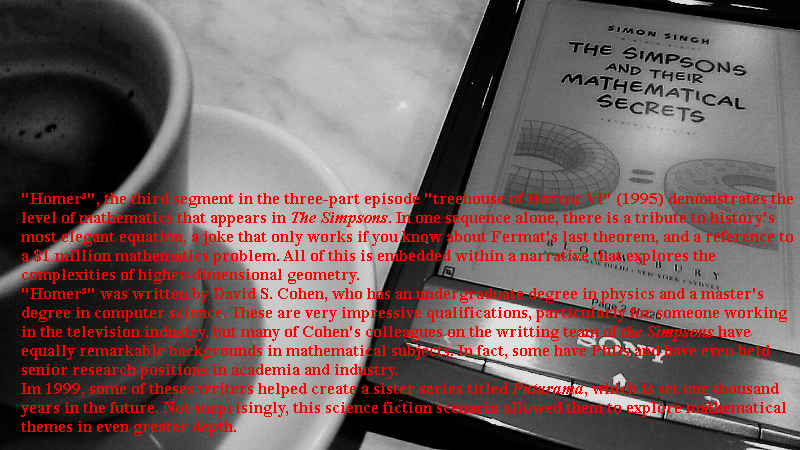
\includegraphics[width=\textwidth]{image5_toRestore}

    \end{subfigure}
    ~ 
        \begin{subfigure}[b]{0.6\textwidth}
        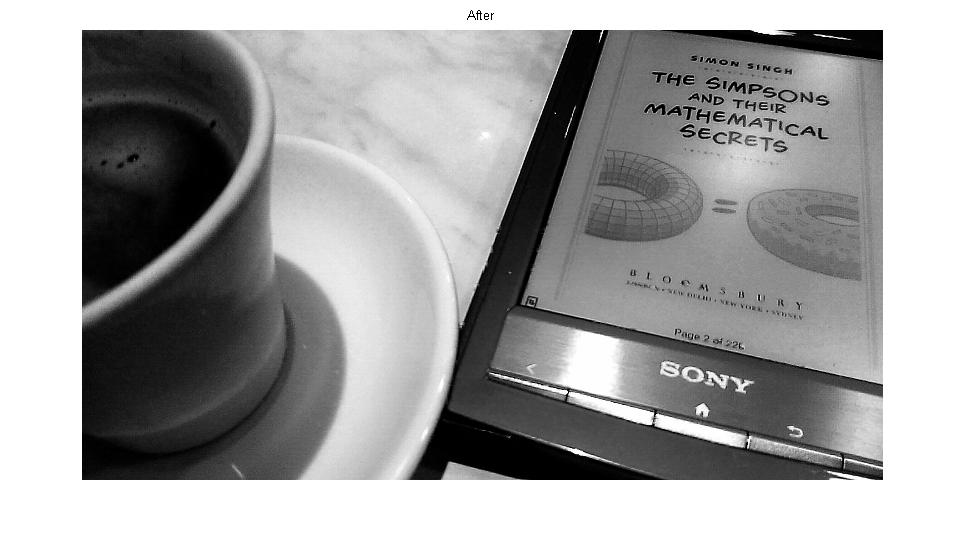
\includegraphics[width=\textwidth]{image5_Restored}

    \end{subfigure}

\end{figure}

\end{frame}


\begin{frame}{Results}
\begin{figure}
    \centering
    \begin{subfigure}[b]{0.5\textwidth}
        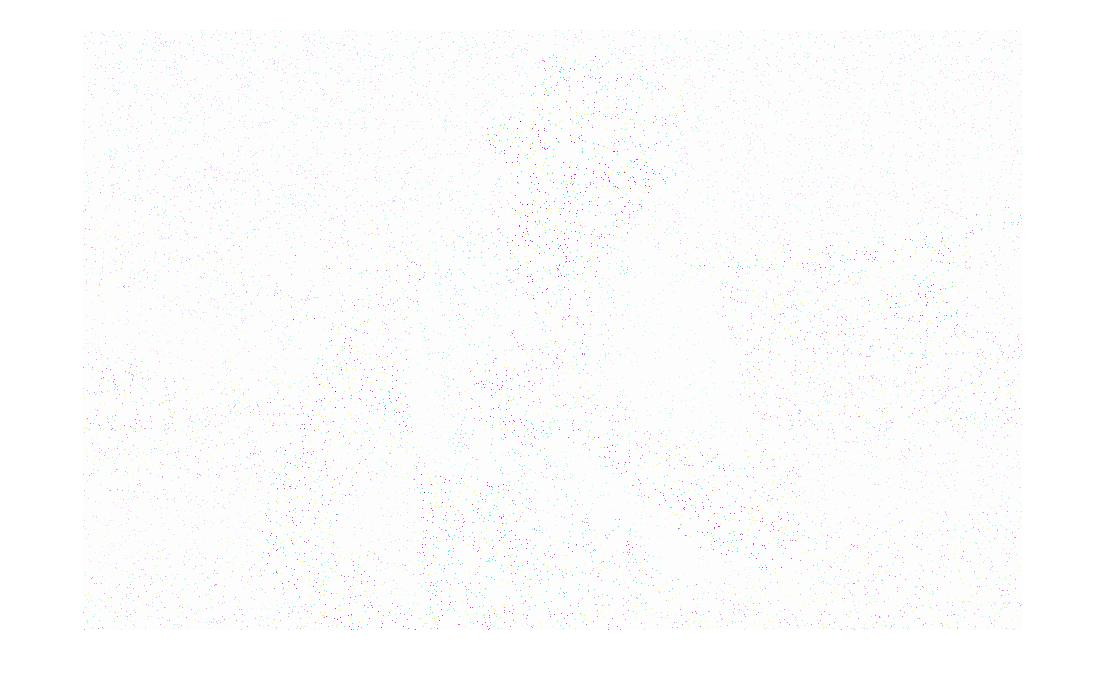
\includegraphics[width=\textwidth]{image6_toRestore_pres}

    \end{subfigure}
    ~ 
        \begin{subfigure}[b]{0.6\textwidth}
        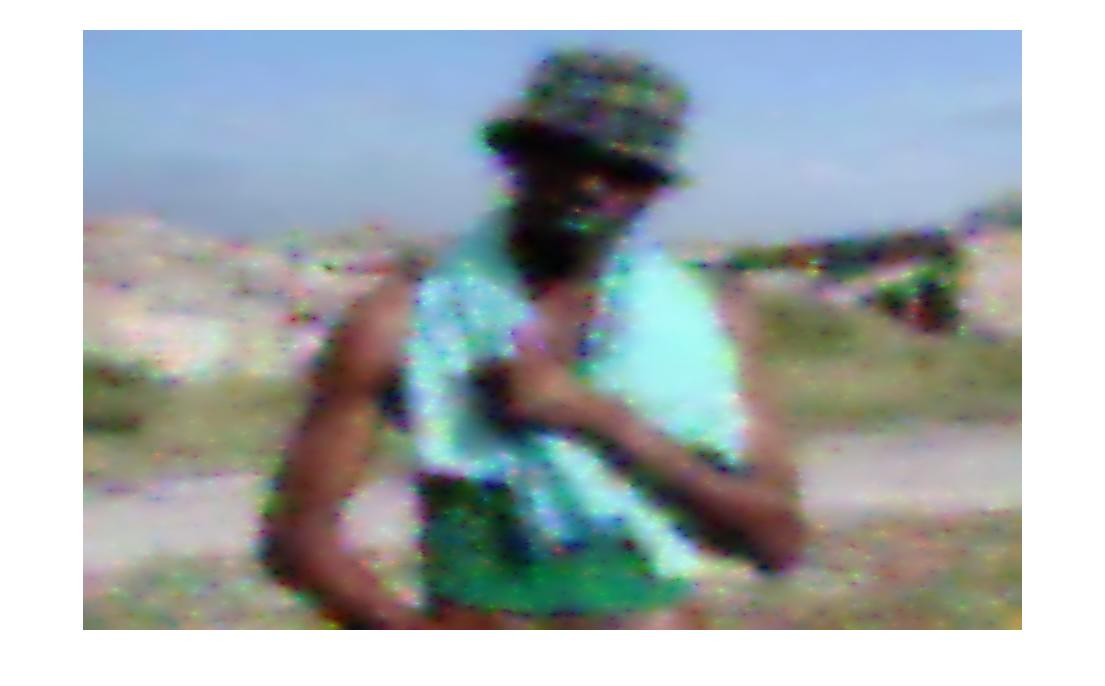
\includegraphics[width=\textwidth]{image6_Restored_pres}

    \end{subfigure}

\end{figure}

\end{frame}


\begin{frame}{Results}
\begin{figure}
    \centering
    \begin{subfigure}[b]{0.45\textwidth}
        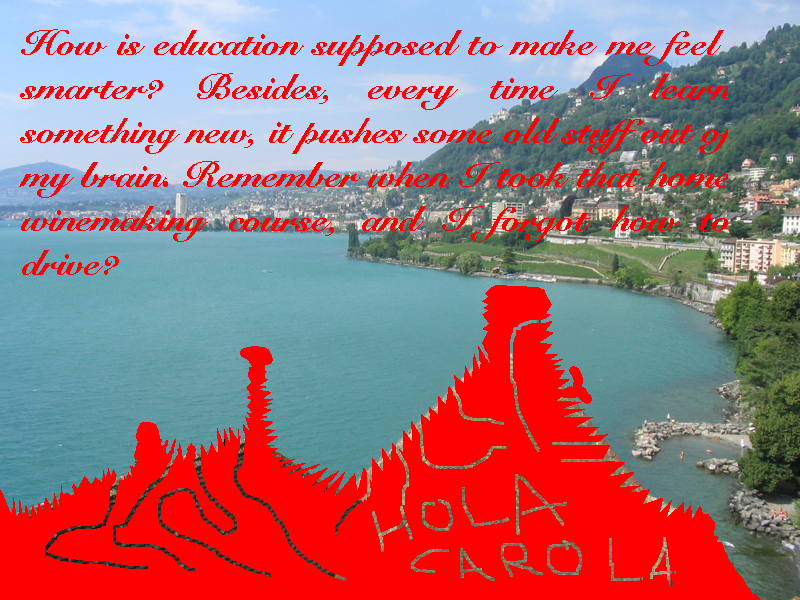
\includegraphics[width=\textwidth]{Image_to_Restore}

    \end{subfigure}
    ~ 
        \begin{subfigure}[b]{0.55\textwidth}
        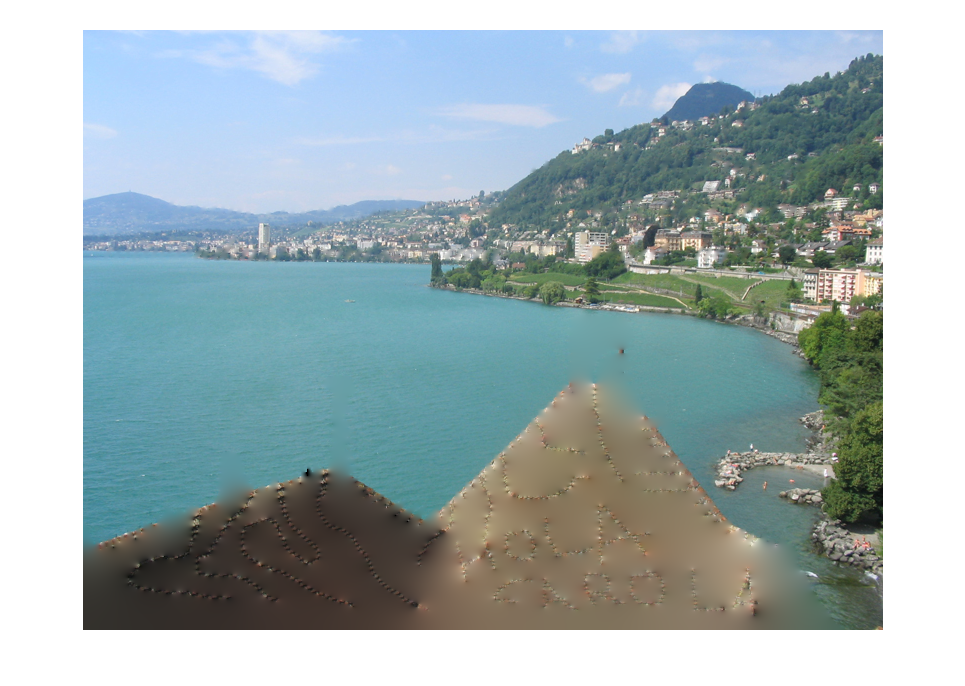
\includegraphics[width=\textwidth]{Image_Restored}

    \end{subfigure}

\end{figure}

\end{frame}

\begin{frame}{Conclusions}
\begin{block}{Conclusions}
\begin{itemize}
\item The inpainted image has a clear definition for the images which we know most of the information.
\item In the image with 99\% information lost, the restored image shows a whole view of the image, but it is not clearly defined.
\item In the goal image, it restores quite well the zone with letters, but not the zone fully painted of red.
\end{itemize}

\end{block}
\end{frame}
\end{document}